\chapter{The Standard Model of particle physics}

The \ac{SM} of particle physics is our current best theoretical framework underpinning our understanding of the subatomic world, providing a description of fundamental elementary particles and their interactions via the electromagnetic force, weak nuclear force and the strong nuclear force. The fourth fundamental force of nature, Gravity, is absent from the SM, highlighting one of its key limitations. However, in high-energy physics experiments, where the interactions of subatomic particles are being studied, the omission of gravity is considered a safe simplification. Extremely powerful predictions have emerged from this theoretical framework, with its greatest success being the discovery of the Higgs boson by the ATLAS and CMS Collaborations in 2012, completing the observational confirmation of all hypothesized SM particles. Despite its success, the Standard Model has its limitations. Along with the absence of gravity, it leaves several fundamental questions unanswered, such as the nature of neutrino oscillations, the existence of dark matter, the hierarchy problem, and the matter-antimatter asymmetry in the universe, which cannot be fully explained by the predicted amount of CP violation, driving the field to look for explanations beyond the SM. In the pursue of \ac{BSM} physics, a deep understanding of the SM theory is crucial. This is the goal of this chapter aiming to establish the base foundation for this work, the SM, by exploring the fundamental blocks of the theory, including its particle content, interactions, and the Higgs mechanism.

\section{Particle content and fundamental interactions}

Built upon the theoretical framework of \ac{QFT}, the SM is a renormalisable theory, where the physical particles observed in nature emerge as quantised excitations of underlying relativistic fields with the interactions between them being themselves being desribed by the exchange of particles. These two groups of particles constitute the particle content of the SM, as shown in Fig~\ref{Figure:Introduction_1}.

\begin{figure}
\centering
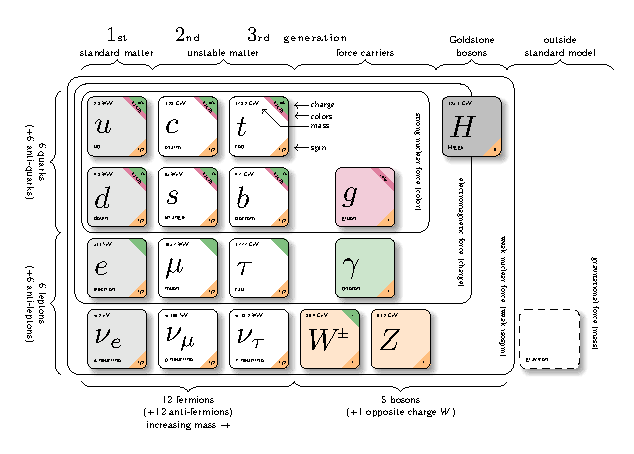
\includegraphics[width= 1\textwidth]{Figures/Introduction/Particles.pdf}
\caption{TODO}\label{Figure:Introduction_1}
\end{figure}

The elementary particles of the SM are fundamental objects which are neither bound states of other particles nor composite. These fundamental constituents of matter, known as fermions, are particles with half-integer spin, and are further split into two types: quarks, that interact via the strong force and leptons which are not.  The electron, the electron-neutrino, the up-quark and the down-quark comprise the first generation of fermions in the SM, whilst the second and third generation fermions are heavier replicas \ie same charge but, different masses. Each SM fermion has a corresponding antiparticle with the same mass but opposite quantum numbers: parity and charge.

The interactions of these matter particles are mediated by the exchange of particles with integer-spin, the gauge bosons. All fermions interact via the weak force, mediated by the exchange of massive vector bosons, the W$\pm$ and the Z bosons. The electrically neutral leptons, neutrinos, do not interact with the massless photon field, $\gamma$, excluding them from the electromagnetic interaction. Only quarks, on the other hand, possess colour charge, coming in three possible states: red, green and blue, allowing them to participate in strong interactions mediated by the exchange of the massless gluon (g). 

\section{Foundation of the fundamental interactions}

In the core of QFT and the SM lies the principle of symmetry, with the Lagrangian density serving as the starting point of describing fundamental interactions. Fundamental laws are closely tied to symmetries, as demonstrated by N\"{o}ether's theorem: a conservation law is implied by the invariance of a Lagrangian under a continuous transformation (symmetry). A striking example of the deep connection between fundamental interactions and symmetry principles is the conversation of angular momentum, defined by a Lagrangian which is invariant under rotational transformations. Built on the principle of local gauge invariance is the SM Lagrangian. Imposing this invariance gives rise to gauge boson fields, whose interactions with the fundamental matter fields are governed by the symmetry group of the gauge transformation. The gauge symmetry group of the SM is

\begin{alignat}{2}
G_{SM} = SU(3)_{C} \otimes SU(2)_{L} \otimes U(1)_{Y}
\end{alignat}

\subsection*{Quantum Chromodynamics}

\ac{QCD} is the theory that describes strong interactions, governed by a $SU(3)_{C}$, with colour charge as the associated quantum number. The mediators of the QCD are the eight massless gluons corresponding to the eight generators of the SU(3) local gauge symmetry. An interesting property of the strong force mediators is that themselves they carry colour charge, allowing them to interact with quarks but, also with themselves. This leads to two characteristic properties of QCD:

\begin{itemize}
    \item Colour confinement: All observed states must be be confined to colour single states, with the absence of free quarks being a direct consequence of this. Quarks in nature are always found in bound states called hadrons.
    \item Asymptotic freedom: At short distances (high energies) the strong interaction weakens, with quarks behaving as quasi-free particles. In contrast, the interaction strengthens at large distances (lower energies) because of colour confinement. 

\end{itemize}

\subsection*{Electroweak theory}

\section{Fundamental forces}
\section{Higgs mechanism}
\section{The Higgs boson}

\cite{Rowling_1997}
\cite{Thor_2011}